\documentclass[12pt, titlepage]{article}

\usepackage{booktabs}
\usepackage{tabularx}
\usepackage{hyperref}
\usepackage{graphicx}
\hypersetup{
    colorlinks,
    citecolor=black,
    filecolor=black,
    linkcolor=red,
    urlcolor=blue
}
\usepackage[round]{natbib}

\newcounter{systnum} %Sistem Test Number
\newcommand{\sthesystnum}{ST\thesystnum}
\newcommand{\sref}[1]{ST\ref{#1}}
\newcounter{utnum} %Unit Test Number
\newcommand{\utheutnum}{UT\theutnum}
\newcommand{\uref}[1]{UT\ref{#1}}

%% Comments

\usepackage{color}

\newif\ifcomments\commentstrue

\ifcomments
\newcommand{\authornote}[3]{\textcolor{#1}{[#3 ---#2]}}
\newcommand{\todo}[1]{\textcolor{red}{[TODO: #1]}}
\else
\newcommand{\authornote}[3]{}
\newcommand{\todo}[1]{}
\fi

\newcommand{\wss}[1]{\authornote{blue}{SS}{#1}} 
\newcommand{\plt}[1]{\authornote{magenta}{TPLT}{#1}} %For explanation of the template
\newcommand{\an}[1]{\authornote{cyan}{Author}{#1}}


\begin{document}

\title{Test Report: EOMEE} 
\author{Gabriela S\'anchez D\'iaz}
\date{\today}
	
\maketitle

\pagenumbering{roman}

\section{Revision History}

\begin{tabularx}{\textwidth}{p{3cm}p{2cm}X}
\toprule {\bf Date} & {\bf Version} & {\bf Notes}\\
\midrule
12-12-2020 & 1.0 & First draft.\\
%Date 2 & 1.1 & Notes\\
\bottomrule
\end{tabularx}

~\newpage

\section{Symbols, Abbreviations and Acronyms}

\renewcommand{\arraystretch}{1.2}
\begin{tabular}{l l} 
  \toprule		
  \textbf{symbol} & \textbf{description}\\
  \midrule 
  T & Test\\
  EOMEE & Equation-of-motion for excited states\\
  SRS & Software Requirements Specification\\
  VnV & Verification and Validation\\
  MG & Module Guide\\
  MIS & Module Interface Specification\\
  \bottomrule
\end{tabular}\\

For more details about symbols, abbreviations and acronyms see 
Sections 1.2 and 
1.4 in \cite{SRS2020}.

\newpage

\tableofcontents

\listoftables %if appropriate

\listoffigures %if appropriate

\newpage

\pagenumbering{arabic}

This document gathers the outcomes of the functional and nonfunctional tests 
described in the System Verification and Validation Plan for EOMEE (VnV) 
[\cite{VnV2020}]. It also serves the purpose of a to-do list of tasks that were 
pending to be completed within the time frame set by the course CAS741.

\section{Functional Requirements Evaluation}
Tests ST1-ST4 (involving the verification of the input formats and 
calculations) were designed to corroborate the functional requirements R1-R5 
specified in the Software Requirements Specification (SRS) (see Section 5.1 in 
VnV and SRS respectively). All tests were completed successfully.

\section{Nonfunctional Requirements Evaluation}

\subsection{Usability}
Section 5.2.1 of the VnV Plan describes the usability test (ST6) 
[\cite{VnV2020}]. This verification remains to be performed by some member of 
the review team (Section 4.1 of the VnV)
		 
\subsection{Accuracy}
The verification of this nonfunctional requirement is covered by the system 
tests ST3, ST4 and ST8 (Sections 5.1.2 and 5.2.3 of the VnV [\cite{VnV2020}]). 
The first two test cases were completed successfully, but ST8 remains to be 
done by Gabriela S\'anchez-D\'iaz.

\subsection{Reusability}
The test designed to verify the modular decomposition of the project is 
described in the VnV Plan section 5.2.2 [\cite{VnV2020}]. It's completion is 
left as a pending task for the author, however, a modification performed in the 
Integrlas modules during the unit testing (reported in Section 
\ref{sec:changes}) could be a preliminary validation of the design.

\subsection{Portability}
This requirement is addressed by test ST5 in the Section 5.2.1 of the VnV Plan 
[\cite{VnV2020}]. The author installed the package in the Ubuntu 20.04 (Focal 
Fossa) and macOS 10.15.7 (Catalina) platforms 
following the installation instruction in the project's repository 
\href{https://github.com/gabrielasd/eomee/tree/cas741}{cas741}. After 
installation the test module was ran. An issue that came up at this point is 
the relative paths of the data files declared in the input files. This problem 
is left ot be resolved by the Gabriela S\'anchez-D\'iaz.
	
\section{Comparison to Existing Implementation}	

%This section will not be appropriate for every project.
To the author's knowledge there aren't existing implementations of EOMEE. 
However, there are electronic structure packages that offer 
similar features to EOMEE (exited states calculation) such as Gaussian 
[\cite{g16}] (commercial) and Psi4 [\cite{psi4}] (open-source). Comparisons 
with the results given by these software remain to be done.

\section{Unit Testing}
All modules described in the Module Guide (MG) and Module Interface 
Specification (MIS) [\cite{MG2020}, \cite{MIS2020}] were tested with the 
exception of the Hardware-Hiding module (M1). The unit tests of EOMEE are 
implemented under the folder \textit{tests/} and 
can be found in the project's GitHub repository 
\href{https://github.com/gabrielasd/eomee/tree/cas741/test}{cas741}

\section{Changes Due to Testing}
\label{sec:changes}
No major issues were detected by the tests. The only change introduced was to 
facilitate the unit testing, in particular this involved the Integrals module 
(Section 8 of MIS). The valid input format of the module was extended to accept 
not only a file path, but also arrays. \\
This modification to the interface of the Integrals module didn't affect the 
remaining modules, therefore it could be considered as a positive indication of 
the modular decomposition of the project (related to the Reusability 
nonfunctional requirement), though this wasn't the actual test designed for 
this requirement (see section 5.2.2 in the VnV Plan [\cite{VnV2020}]). 

\section{Automated Testing}
The unit testing framework used was \href{https://docs.pytest.org/en/stable/} 
{Pytest}. Also, a \href{https://travis-ci.org/}{Travis-CI} .yaml file was set 
up for automated 
testing, however currently the buildup fails due to code formatting standards 
errors detected by the Python linters (specified in section 4.5 in the VnV 
Plan [\cite{VnV2020}]).

		
\section{Trace to Requirements}
The original table for the trace between requirements and tests can be found in 
section 5.3 of the VnV Plan [\cite{VnV2020}].
\begin{table}[ht]
	\centering
	\begin{tabular}{|l|c|c|c|c|c|c|c|c|}
		\hline
		& ST1& ST2& ST3& ST4& ST5& 
		ST6& ST7& ST8\\	\hline	
		R1& X& & & & & & &\\ \hline
		R2&  & X& & & & & &\\ \hline
		R3&  & X& & & & & &\\ \hline
		R4&  &  & X& X& & & & \\ \hline
		R5&  &  & X& X& & & &\\ \hline
		Reusability& & & & & & &  X& \\ \hline
		Usability& & & & &   X& X& &\\ \hline
		Portability& & & &   & X& && \\ \hline
		Accuracy& & & X& X&  &  & & X\\ \hline
	\end{tabular}
	\caption{Traceability for system tests and requirements}
	\label{table:traceab}
\end{table}
		
\section{Trace to Modules}	

Table~\ref{table:moduletraceab} shows the trace between EOMEE modules and 
unit tests. The modules outside of the unit testing scope are discussed in 
Section 6.1 of the VnV Plan [\cite{VnV2020}].

\begin{table}[ht]
	\centering
	\begin{tabular}{l|c|c|c|c|c|c|c|c}
		\hline
		&M1& M2& M3& M4& M5& M6-M11& M12& M13\\	\hline	
		UT1-UT2&  & & X& & & &&\\ \hline
		UT3-UT5&  & & &X & & &&\\ \hline
		UT6-UT9&  & & & &X & &&\\ \hline
		UT10&  & & & & & &X&\\ \hline
		UT11&  & & & & & &&X\\ \hline
	\end{tabular}
	\caption{Traceability for modules and unit test sections}
	\label{table:moduletraceab}
\end{table}	

\section{Code Coverage Metrics}
Figure~\ref{coverage} shows the coverage statistics for EOMEE. The ``Missing" 
column indicates lines of code left untested, these involve abstract methods of 
the EOM module interface and some conditional statements related to the 
selection of the EOM methods in the Control and Output modules. These lines 
were not deemed critical for the successful execution of the program and that 
is 
way were left uncovered. It remains as a future task to get 100\% code 
coverage.
\begin{figure}[h!]
	\centering
	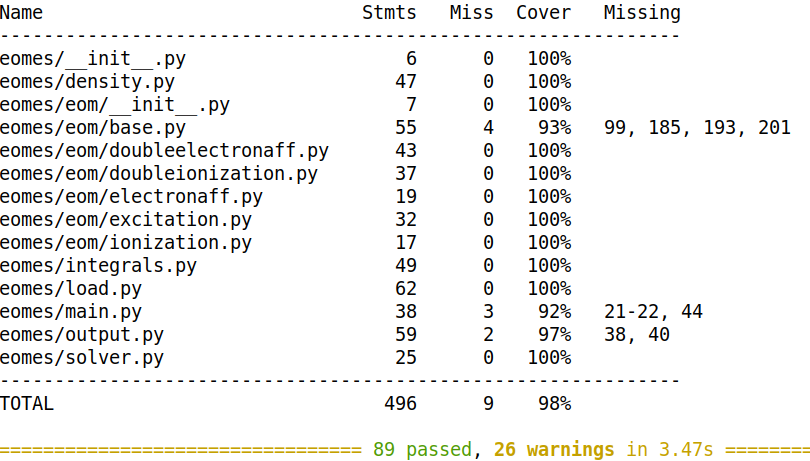
\includegraphics[width=0.7\textwidth]{coverage.png}
	\caption{Code Coverage of EOMEE tests}
	\label{coverage}
\end{figure}

\bibliographystyle{plainnat}

\bibliography{../../refs/References}

\end{document}